\section{Results and Discussion}

\iffalse
\begin{figure}[t]
\centering
\includegraphics[width=3in]{perturb}
\caption{After perturbation, the self-union of \emph{Bunny} with QuickCSG still suffers from topology problem. The green boundary faces indicate topological deficiencies.}
%
\label{fig:boundaryedge}
\end{figure}

\begin{figure}[t]
\centering
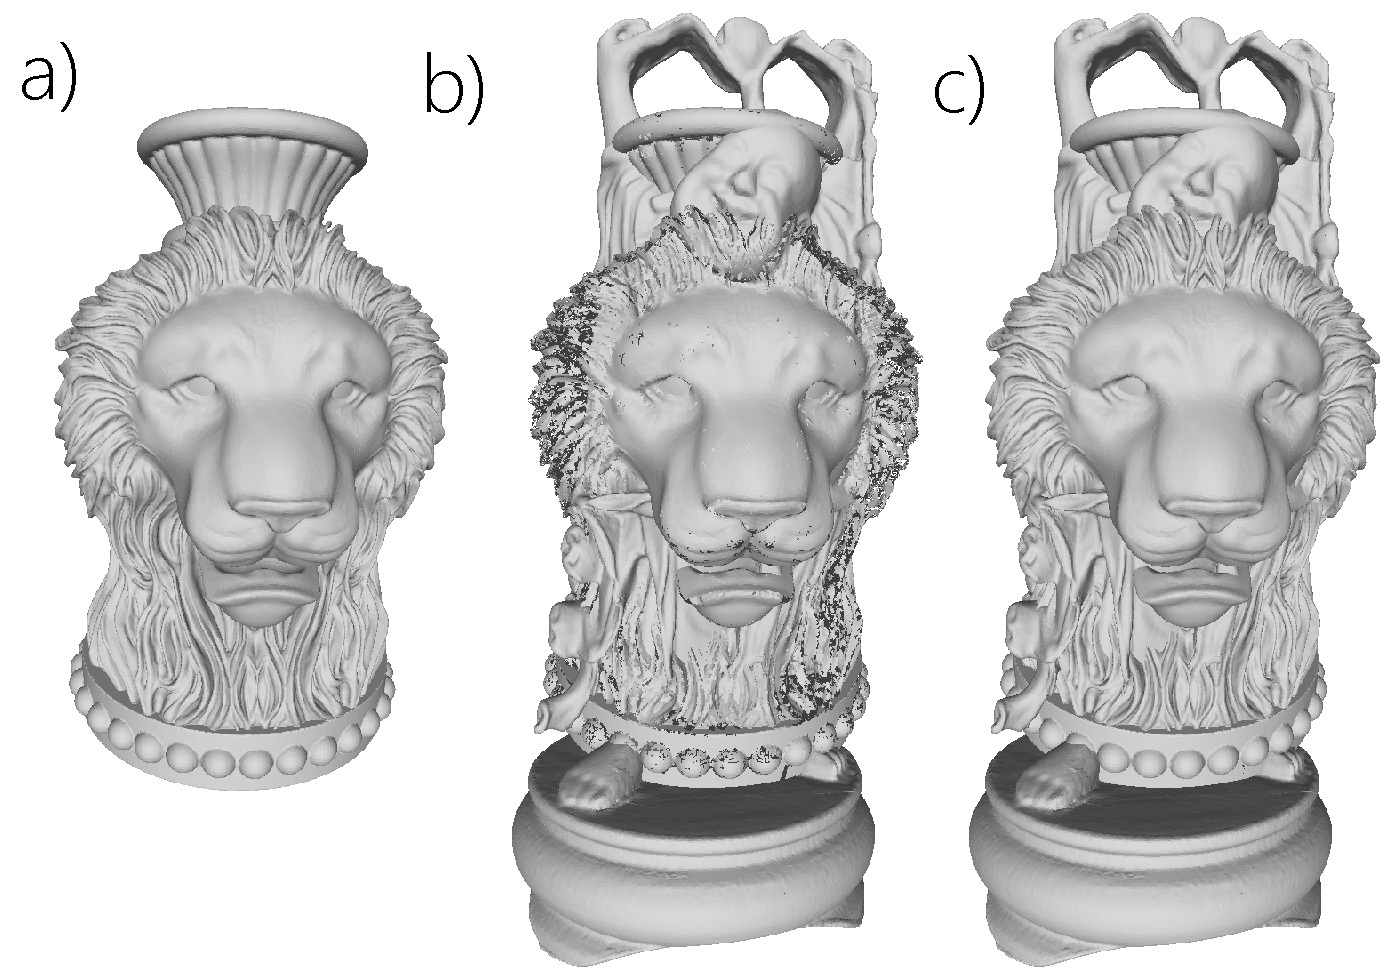
\includegraphics[width=3in]{buddalion}
\caption{ Results from $Budda\cup Lion$: a) incorrect result using CGAL, b) incorrect result using Cork, and c) correct result using our method. }
%.
\label{fig:buddalion}
\end{figure}
\fi
%We implemented the proposed method in C++ and tested a series of models on a laptop with Intel Core i5 1.5GHz CPU and 8GB RAM. To prove  both the efficiency and robustness, we perform boolean evaluation on various CSGs with different complexity. We also compared our method with several previous works with available implementations, including CGAL \cite{cgal:hk-bonp3-15a}, Maya \cite{Maya2015,barki2015exact},"Cork" \cite{Cork}, "QuickCSG" \cite{douze2015quickcsg}, "Carve" \cite{Carve}, and online service of Campen and Kobbelt's plane-based method \cite{campen2010exact,WebBSP}.

We implemented our proposed method in C++, and tested a series of models on a PC with an Intel Core i5 CPU and 8 GB of RAM. We compared our method with several existing methods, including CGAL \cite{cgal:hk-bonp3-15a}, Cork  \cite{Cork}, QuickCSG \cite{douze2015quickcsg}, Carve \cite{Carve}, and online service of Campen and Kobbelt's plane-based method \cite{campen2010exact,WebBSP}. Among them, CGAL and Carve use exact arithmetic. To ensure fairness, we turn off any features of multi-thread computation during the comparison.
%Also, the self-intersection tests of meshes are performed using an open-source library VCG \cite{VCG}.



\subsection{Self-Union on Thingi10K Dataset}

\begin{figure}[t]
\centering
\includegraphics[width=3.5in]{total3}
\caption{The performance of test on Thingi10k (top) and Barki et al.'s dataset (bottom). We outline the median of processing time for each method. The different histogram areas result from the different success rate.}
\label{fig:total}
\end{figure}



\begin{figure}[t]
\centering
\includegraphics[width=3.5in]{cleanness}
\caption{The result meshes of our method for the self-union of Thingi10k are cleaner than state-of-art methods. The Cork and QuickCSG assume general position and cannot handle self-union at all, so they failed to produce solids in most of the cases.}
\label{fig:cleanness}
\end{figure}


\begin{figure}[t]
\centering
\includegraphics[width=3.5in]{profile3}
\caption{Performance profile of tests on Thingi10k (top) and Barki et al.'s dataset (bottom). The red, yellow, green, blue areas represent the time percentage of octree construction, intersection computation, tessellation and classification, respectively. Each one-pixel column represents a test. All the tests are sorted by total processing time.}
\label{fig:profile}
\end{figure}

\begin{figure}[t]
\centering
\includegraphics[width=3in]{scatter}
\caption{For the self-union tests on Thingi10k, the linear relation between processing time and triangle number is apparent.}
\label{fig:scatter}
\end{figure}


\begin{figure}[t]
\centering
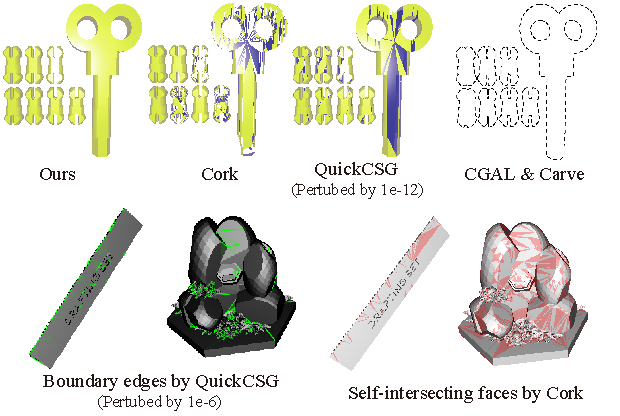
\includegraphics[width=3.2in]{comp}
\caption{\emph{First row}: the results of self-union of \emph{components}. QuickCSG (adding perturbation of 1e-12) and Cork cannot produce valid results. CGAL and Carve simple crashed and do not give a result. \emph{Second row}: In our self-union tests, QuickCSG tends to produce results with many boundary edges (green lines), and Cork tends to produce many self-intersecting faces (red faces).}
\label{fig:perturb}
\end{figure}


\begin{figure}[t]
\centering
\includegraphics[width=3.0in]{boolean-11}
\caption{After coordinates approximation, the 'thin' triangle in the middle intersect adjacent faces and results in self-intersection on the mesh (red triangles).}
\label{fig:roundoff}
\end{figure}



We reproduce the experiments of \cite{zhou2016mesh} on the Thingi10K dataset on website thingiverse.com. The dataset currently contains 9956 .stl models, which are heavily biased towards 3D printing modeling by amateurs or semi-professionals. Since .stl models are triangle streams rather than meshes, we merge the exact coincident vertices to reconstruct connectivity. After that, we check the cleanness of all of the models. Among the 9956 meshes, 4509 meet the requirements of solid. The face numbers of these meshes generally follows a log-normal distribution with the average of 17k. We limit our comparison to these solid meshes.

The comparison results are available for CGAL, Cork, Carve and QuickCSG. Web service of Campen et al. \cite{campen2010exact,WebBSP} does not support batch processing. Therefore, we made a few tests manually, and roughly a half of them failed. The implementation of recent works \cite{zhou2016mesh,barki2015exact} are not available. Both methods are based on exact arithmetic. The performance of method in \cite{zhou2016mesh} is claimed to be close to Carve (with parallel computation) by the results on the same dataset Thingi10k in their paper.

The computation time of our method outperform most of other methods (see Fig. \ref{fig:total} \emph{top}). Even compared with the fastest QuickCSG, which is not exact, our method takes only about two times of the processing time. We profile each stage of our method, and the results indicate the bottleneck is the intersection computation (see Fig. \ref{fig:profile} \emph{top}). Also, from Fig. \ref{fig:scatter}, the linear relation between triangle number and processing time implies the ability of our method to handle large boolean evaluations.

Our method produces results in 98.8\% of the tests. The cleanness of resulting meshes are tested by checking self-intersecting (we use VCG \cite{VCG}) and the total signed incidence of every edge \cite{zhou2016mesh}. If the total signed incidence of every edge of a mesh is zero, then the mesh is a piecewise-constant
integer \emph{generalized winding number} (PWN) \cite{zhou2016mesh} mesh. These two requirements are sufficient conditions of solid. According to Fig. \ref{fig:cleanness}, over 80\% of our results are solids, which outperform all other methods. We also notice very low rates of success for Cork and QuickCSG. This is because both methods assume general position, which is not the case for self-union. Even after perturbation, they can hardly produce solid results (see Fig. \ref{fig:perturb}).

The failure cases and unclean results of our method do not impair the robustness of our algorithms. The reasons lie on the degenerate faces and close-to-degenerate faces from the inputs. The normal vectors of degenerate faces cannot be defined so face classification may fail when encounter such faces. Also, close-to-degenerate faces can become degenerate faces or lead to self-intersecting (see Fig. \ref{fig:roundoff}) after conversion to their P-reps. This is because the conversion method \cite{campen2010exact} requires coordinates rounding-off. In our implementation, the IEEE-754 single-precision floating-point coordinates (precision=24) are rounded to the precision of 18$\scriptsize{\sim}$20.

\subsection{Binary Boolean Operations}

\iffalse

\begin{table*}[ht]
\caption{Computation time statistics of binary boolean operations (seconds)}
\label{tab:performance}
\centering
\begin{tabular}{*{9}{c|}c}%*{4}{>{\centering\arraybackslash}p{35pt}}}
\hline
{No.} & {Model} & {Face Num. 1} & {Face Num. 2} &
CGAL & Maya & Cork & Carve & QuickCSG & Our Method
\\
\hline\hline
1 & Budda $\cup$ Lion & 1.08M & 400k & - & - & - & - & 3.44 & 4.30\\
2 & Dragon $\cup$ Bunny & 100k & 70k & - & - & - & - & 0.613 &1.12 \\
3 & Armadillo $\cup$ Armadillo2 & 150k & 150k & 487 & 15.4 & 7.00 & 189 & 0.746 & 1.33\\
4 & Horse $\cup$ Corpse & 145k & 499k & - & 38.6 & 12.6 & 1.52k & 0.630 & 0.980 \\
5 & Budda $\cup$ Budda2 & 1.08M & 1.08M & - & - & - & - & 4.84 & 7.73\\
\hline
\end{tabular}
\begin{flushleft}

\end{flushleft}
\end{table*}

\begin{figure}[t]
\centering
\includegraphics[width=3.5in]{total2}
\caption{a) There is ambiguity as to the orientation of the loop in this tess-graph. b) When there is more than one connected component in a tess-graph, auxiliary intersections (yellow line) are used to connect the components.}
\label{fig:profile2}
\end{figure}


\fi


The most common situations of boolean evaluations in CAD are binary evaluations. It is because people are used to incrementally refine their models by adding or subtracting one shape each time. Although our method is variadic, we perform comparisons of binary boolean evaluations. We reproduce the experiments in \cite{zhou2016mesh} on the dataset of Barki et al. \cite{barki2015exact}. The dataset of Barki et al. contains 26 triangle meshes. All of them are closed and manifold, and 10 of them contain local self-intersecting. We exhaustively perform union, intersection, and both asymmetric differences for all pairs, producing $26\times(26-1)/2 \times 4=1300$ results.

The configuration of such tests satisfy the general position assumption, so Cork and QuickCSG can produce correct result in more cases than during self-union tests. But we address that such tests are performed only for completeness and coplanar faces are important situations in CSG modeling. The results (see Fig. \ref{fig:total} \emph{bottom}) shows that our method is slightly slower than QuickCSG, and much faster than other exact methods. We notice the bottleneck shifts from intersection computation to octree construction in this time (see Fig. \ref{fig:profile} \emph{bottom}). This is because compared with self-union tests, the binary boolean evaluations generally process fewer intersections. We also find that Carve has shows much worse performance in these cases than in self-union tests, which indicates that Carve does not localize the boolean evaluations within intersection areas.

\subsection{Variadic Boolean Operations}


\begin{table*}[ht]
\caption{Computation time statistics of the evaluations of large CSGs (seconds)}
\label{tab:performance2}
\centering
\begin{tabular}{*{12}{c|}c}%*{4}{>{\centering\arraybackslash}p{35pt}}}
\hline
\multirow{2}{*}{No.} & \multirow{2}{*}{Model} & \multirow{2}{*}{\tabincell{c}{Face \\ Num.}} & \multirow{2}{*}{\tabincell{c}{Mesh \\ Num.}} & \multirow{2}{*}{\tabincell{c}{CGAL \\ \cite{cgal:hk-bonp3-15a}}}
& \multirow{2}{*}{\tabincell{c}{Cork \\ \cite{Cork}}} & \multirow{2}{*}{\tabincell{c}{Carve \\ \cite{Carve}}} & \multirow{2}{*}{\tabincell{c}{QuickCSG \\ \cite{douze2015quickcsg}}}&
\multicolumn{5}{c}{Our Approach$^\dag$}\\
 \cline{9-13}
 &&&&&&&& Total & Step 1 & Step 2 & Step 3 & Step 4\\
 \hline\hline
 1 & Organic & 219k & 6 & - & 14.3 & 63.1 & 0.580 & 2.75 & 0.892 & 1.32 & 0.397 & 0.118\\
 2 & T1 & 80k & 50 & 1.00k & 18.5 & 10.4 & 0.388 & 14.4 & 0.691 & 2.71  & 8.11 & 2.87\\
 3 & T2 & 7k & 50 & 2.81k & - & 16.0 & 0.804 & 5.52 & 0.162 & 1.11 & 3.29 & 0.746\\
 4 & Sprocket & 11k & 52 & 211  & - & 4.26 & (0.132)* & 0.386 & 0.093 & 0.105 & 0.149 & 0.034\\
 5 & Ring \& Ball & 146k & 801 & -  & - & 187 & (1.10) & 20.0 & 1.04 & 3.55 & 8.61 & 6.68\\
 \hline
 \end{tabular}
 \begin{flushleft}
   $^\dag$ ~~The \emph{step 1, 2, 3, 4} are octree constrcution, intersection computation, tessellation and classification respectively.

 * ~~The bracket indicates that although QuickCSG gives the answer, the result meshes are full of topology deficiencies that contain thousands of boundary edges.
 \end{flushleft}
 \end{table*}

\begin{figure*}[t]
\centering
\includegraphics[width=7in]{multi}
\caption{The result meshes of our method for variadic boolean evaluations. From the left to the right is Organic, T1, T2, Sprocket and Ring \& Ball respectively. The performance of our method is better on cases with loosely distributed primitives (T2, Sprocket, Ring \& Ball).}
\label{fig:multi}
\end{figure*}


To identify the ability of the methods to evaluate large CSGs, we reproduce the experiments of Douze et al. \cite{douze2015quickcsg}. Some of variadic test cases are not presented because of the 8GB memory limitation. Since only QuickCSG and our method are variadic, comparisons with the other methods are performed by decomposing CSG into binary boolean operations. We also add an extreme CSG with 801 primitives to prove the effect of label caching (\S\ref{sec:acc}).

The performance of our method  (see Table \ref{tab:performance2}) is not that good in these cases, because our method exhaustively compute all intersections between primitives, which is not necessary. The QuickCSG is much faster than our method, but generally produces results with worse qualities. Except QuickCSG, our performance is better than other methods in most time. The evaluation time of \emph{Ring} \& \emph{Ball} is 38.1s in our first try. We find that each primitive usually intersects with less than 10 other primitives. Therefore, we applied the label caching, and the total computation time drops to only half of the original.

\subsection{Implementation}
\label{sec:esubroutine}

\begin{figure}[t]
\centering
\includegraphics[width=3.5in]{boolean-06}
\caption{a) We construct an auxiliary connection to connect each inner component with outer component (the red line segment). By checking the intersections on the auxiliary connection, we find that the orange loops are identical.  b) We construct the P-rep of the auxiliary connection by $\bm{v}_o$ and the exact coordinates of the end points of $\bm{e}$. }
\label{fig:dual}
\end{figure}


\vspace{0.5em}
\noindent\textbf{Tess-graph with multiple components. }
There is no guarantee that the tess-graph will be a connected graph. If a tess-graph contains more than one connected component, we need to merge identical valid loops, which allows us to generate polygons with non-zero genus. To find identical loops, we construct an auxiliary connection $C_{ext}$ for each inner component, which connects a vertex $\bm{v}_o$ on the outer component and a vertex $\bm{v}_i$ on the current inner component (see Fig. \ref{fig:dual}a). After that, we search all the connections belongs to the current inner component that intersection $C_{ext}$, and find the one (as $C_1$) which is the nearest to $\bm{v}_o$. Then we search all the connections not belongs to the current inner component that intersection $C_{ext}$, and find the one (as $C_2$) which is the nearest to $C_1$. Finally, by figuring out in which valid loops $C_1$ and $C_2$ are, we find the identical pair of loops.

To guarantee that $C_{ext}$ has an exact P-rep within double-precision, the vertex of triangle is chosen as the $\bm{v}_o$. On the other hand, $\bm{v}_i$ must be the vertex generated by the intersection between an triangle and an edge (as $\bm{e}$). All intersection points introduced by triangle-triangle intersections are of this type. In this way, we obtain three vertices with exact coordinates ($\bm{v}_o$ and the two end points of $\bm{e}$). Therefore, we can construct the plane on which $C_{ext}$ lies by the same method of generating supporting planes of triangle faces (see Fig. \ref{fig:dual}b).

\vspace{0.5em}
\noindent\textbf{Seed label generation. }
The label vector of the seed vertex can be generated by a point-in-polyhedron test \cite{ogayar2005point}, using the octree as an acceleration structure \cite{frisken2002simple}. However, a simpler strategy can be adopted which chooses a vertex with known labels as the seed. The inclusion labels of vertex with the maximum $x$-coordinate are either $out$ ($in$, if the complement is applied on the mesh) or $on$. The $on$ labels can be determined by connectivity. Exceptions can occur because of our ignorance of coplanar situations---vertices may not be added to the primitive, even if they are on surface of it. Fortunately, if seed vertex is chosen whose neighboring faces are not all coplanar, exceptions can be avoided.

Label vectors can propagate within a certain mesh, and between different meshes across shared edges. Therefore, in most cases, only a single seed vertex is needed for classification. However, if there are more than two connected components among the tessellated meshes, extra seeds are required. The labels of these additional seeds have to be computed by point-in-polyhedron tests.

\vspace{0.5em}
\noindent\textbf{Exporting to float-point number. }
The vertices of the final mesh are represented as either planes or vertex coordinates. The vertices originating from the input meshes have exact coordinates, and the vertices newly introduced by the intersection between meshes have only P-reps, and require round-off when computing their coordinates. Although our method guarantees the correct topology in the final mesh, round-off errors can still cause topological deficiencies. This is called \textbf{vertex rounding} problem. We can adopt the method of Zhou et al. \cite{zhou2016mesh} to solve this problem iteratively. For the consideration of efficiency, we do not include this step during our comparison experiments.

\subsection{Limitations and Future Work}

We found that performance of our method was poor for CSGs that contained a lot of meshes within a small area (Table. \ref{tab:performance2}, \emph{T1}). In these cases, our method computes many intersections that will not appear as edges in the final mesh, leading to unnecessary tessellation. Optimization may be explored to alleviate this problem.

The inputs of our method are limited to solids. However, recent work \cite{zhou2016mesh} have proposed that the piecewise-constant integer \emph{generalized winding number} (PWN) is a more powerful method to identify the insides and outsides of meshes. The input requirements of our method may be extended to PWN meshes, that allow self-intersection. We believe that this would be an interesting and valuable extension of our work.

\section{Summary}

In this paper, we propose a novel boolean method. Our method can efficiently perform variadic boolean operations, and is robust with solid inputs. The novel component of our approach is to combine P-reps with V-reps. P-reps allow us to strictly follow the principle of no geometry construction to avoid numerical errors ,and the V-reps enables coarse tests and fast neighborhood queries to reduce the need of slow plane-based computation. The experimental results show that the performance of our method is competitive with state-of-the-art non-robust methods, while guaranteeing robustness under consistent inputs.
